\begin{apendicesenv}
\partapendices

\chapter{Termo de Abertura de Projeto}
\label{project_charter}

\begin{table}[h!]
\centering
\caption{Histórico de Versão}
\label{my-label}
\begin{tabular}{|l|l|l|l|}
\hline
\textbf{Data} & \textbf{Versão} & \textbf{Descrição}   & \textbf{Responsável} \\ \hline
24/03/2017    & 1.0             & Criação do Documento & Nicolas Boarin       \\ \hline
\end{tabular}
\end{table}

\section{Nome do Projeto}
Bicicleta Elétrica com Dispositivo de Auxílio à Rota

\section{Descrição do Projeto}
A proposta visa a criação de uma bicicleta elétrica com um sistema embarcado acoplado em sua estrutura. Este sistema embarcado quando sincronizado a um aplicativo de mapeamento GPS (que em parte será desenvolvido pelo grupo utilizando a API do Google Maps) irá mostrar ao ciclista com sinais visuais e tácteis a rota escolhida pelo mesmo no aplicativo, sem a necessidade de tirar o foco da estrada para verificar de forma contínua a rota pelo celular.

\section{Objetivos do Projeto}
Este projeto tem por objetivo uma redução do uso contínuo do celular, ao se usar um veículo (no caso abordado uma bicicleta elétrica),  a fim de um aumento da atenção do ciclista a sua rota desejada.

Dado o contexto no Brasil um dos objetivos secundários do projeto é que com a diminuição da frequência de uso do dispositivo móvel por um usuário do produto, isso poderá a diminuir as chances do mesmo poder a vir ser assaltado.

\textbf{Objetivos Gerais:}
\begin{itemize}
  \item Criação de uma bicicleta elétrica;
  \item Criação de um aplicativo para se “comunicar” com a bicicleta;
  \item Criação de um suporte na bicicleta para os componentes eletrônicos;
  \item Criação de um módulo de guia de rota GPS;
  \item Integração do módulo de guia no suporte da bicicleta e a sincronização com o app. 
\end{itemize}

\section{Justificativa do Projeto}
“As conversas de telefone celular tendem a restringir artificialmente a percepção periférica medida por um campo visual. Isso sugere que o uso do telefone celular durante a condução pode diminuir o campo visual perceptivo, tornando o condutor menos consciente do ambiente e mais suscetível a acidentes.” \cite{maples2008effects} 

	Tendo essas informações o projeto foi proposto a fim de reduzir a frequência de uso de um aparelho móvel enquanto o veículo elétrico estiver em movimento, assim aumentando a percepção do usuário ao seu redor, assim diminuindo o número de acidentes e respectivos assaltos causados por uma possível menor visibilidade do celular.

\section{Recursos do Projeto}
A solução proposta possui os seguintes recursos:
\begin{itemize}
	\item Aplicativo para dispositivo móvel de escolha a rota GPS;
	\item Sistema de retroalimentação de energia por pedaladas;
	\item Módulo de luzes guias para a rota selecionada;
	\item Motor e controladores instalados na bicicleta.
\end{itemize}

\section{Subprodutos Identificados}
A solução apresentada possui os seguintes subprodutos:

\begin{itemize}
	\item Aplicação de Dashboard Interativa - O aplicativo criado pelo grupo possuirá como funcionalidade principal a escolha da rota, mas também contará com funções como uma dashboard de acompanhamento das viagens do usuário com métricas como "Km percorridos" e "Tempo gasto por rota".
	\item Estrutura Física da Bicicleta - A bicicleta será projetada a fim de manter o centro de massa no centro, sua estrutura também será designada a ponto de tentar maximizar a vida útil de todos os componentes eletroeletrônicos de riscos como vibração, temperatura e exposição ao Sol. 
\end{itemize}

\section{Stakeholders}
Qualquer tipo de pessoa que seja envolvida no projeto de alguma forma, seja no próprio desenvolvimento, no auxílio, ou mesmo uso do produto final foram considerados stakeholders.  A tabela abaixo mostra os stakeholders identificados pelo grupo:

\begin{table}[h!]
\centering
\caption{Stakeholders}
\label{my-label}
\begin{tabular}{|p{3cm}p{6cm}p{6cm}|}
\hline
\multicolumn{1}{|l|}{\textbf{Nome}} & \multicolumn{1}{l|}{\textbf{Descrição}}               & \textbf{Responsabilidades}                                             \\ \hline
Integrantes do Projeto              & Integrantes do grupo de desenvolvimento do projeto    & Produzir, analisar, verificar, acoplar módulos e validar produto final \\
Professores de PI2                  & Professores da disciplina de PI2                      & Verificar o andamento do projeto e auxiliar e por fim avaliar o mesmo  \\
Usuários de Teste                   & Pessoas que utilizarão os protótipos feito pelo grupo & Utilizar o protótipo a fim de dar feedback sobre possíveis melhorias   \\
Usuários Finais                     & Pessoas que utilizarão o produto final                & Usufruir do projeto em seu dia a dia                                   \\ \hline
\end{tabular}
\end{table}


\section{Líderes do Projeto e Suas Responsabilidades}
Sendo um projeto integrador, cada engenharia terá até uma certa parte seu trabalho feito de forma que cada frente de uma determinada engenharia possua autonomia. Cada um dos grupos de uma engenharia específica possuirão um representante para se comunicar com outros líderes. 

Os líderes ficam responsáveis pela área de gerenciamento e auxílio de cada time que ele está encarregado e também como representante de sua área caso outro grupo possua uma dependência da área na qual o mesmo atua. 

Após as escolhas dos devidos líderes a lista atualizada de líderes e suas áreas é:

\begin{itemize}
	\item Frente Estrutural/Mecânica - Marlos Pereira
	\item Frente Eletromecânica - Rodrigo Araújo
	\item Frente Eletroeletrônica - Bruno Fares
	\item Frente Software - Levi Moraes
	\item Frente Energia/Alimentação - Karine Ximenes
\end{itemize}

\section{Cronograma de marcos sumarizado}
Os principais marcos do projeto, juntos com suas descrições e respectivos responsáveis foram detalhados  na tabela abaixo:  

\begin{table}[]
\centering
\caption{Macro Cronograma}
\resizebox{\textwidth}{!}{
\label{my-label}
\begin{tabular}{|p{2cm}|p{4cm}|p{11cm}|}
\hline
\textbf{Data}         & \textbf{Marcos}                                                                    & \textbf{Descrição}                                                                                                                                                                                                                                        \\ \hline
17/03/17              & \begin{tabular}[c]{@{}l@{}}Proposta Inicial\\ e Formação do \\Grupo\end{tabular}     & \begin{tabular}[c]{@{}l@{}}Definição em aula sobre a ideia do projeto de forma\\ abstrata junto com os integrantes que irão compor o grupo\end{tabular}                                                                                                   \\ \hline
18/03 $\sim$ 24/03/17 & Refinamento da proposta                                                            & \begin{tabular}[c]{@{}l@{}}Reuniões entre o grupo para criar uma visão\\ compartilhada sobre o projeto\end{tabular}                                                                                                                                       \\ \hline
05/04 $\sim$ 07/04/17 & Ponto de Controle 1                                                                & \begin{tabular}[c]{@{}l@{}}Apresentação do grupo sobre a concepção do projeto,\\ já com a ideia bem definida sobre o escopo do mesmo\\ e requisitos bem refinados, a fim de mostrar o que será\\ desenvolvido no projeto para os professores\end{tabular} \\ \hline
08/04 $\sim$ 25/05/17 & Criação dos Módulos Específicos                                                    & \begin{tabular}[c]{@{}l@{}}Cada grupo ficará encarregado da criação de seus \\respectivos módulos/componentes\end{tabular}                                                                                                                                \\ \hline
31/05 $\sim$ 02/06/17 & Ponto de Controle 2                                                                & \begin{tabular}[c]{@{}l@{}}Apresentação dos componentes de cada engenharia\\ para a banca avaliadora junto com o andamento do \\projeto\end{tabular}                                                                                                        \\ \hline
04/06 $\sim$ 29/06/17 & \begin{tabular}[c]{@{}l@{}}Integração de \\Componentes e  \\Homologação\end{tabular} & \begin{tabular}[c]{@{}l@{}}Integração dos módulos de cada engenharia a fim\\ de entregar o produto final com todos seus respectivos teste\end{tabular}                                                                                                    \\ \hline
05/07/17              & Ponto de Controle 3                                                                & \begin{tabular}[c]{@{}l@{}}Apresentação do produto final para a bancada \\avaliadora, mostrando os respectivos testes definidos de \\acordo com os requisitos definidos pelo grupo.\end{tabular}                                                           \\ \hline
\end{tabular}
}
\end{table}

\section{Investimento Preliminar}
Como ainda não foi definida uma estrutura ideal para o projeto, uma estimativa precisa sobre o preço não pode ser dada, mas o grupo avaliou que para um investimento inicial cada integrante teria teria que entrar com R\$ 100,00, tirando o motor elétrico que um integrante já possuía (estimado em R\$ 500,00), então o valor preliminar foi definido como R\$ 1.800,00.

\section{Restrições e Riscos}
Os riscos inicialmente apontados pela equipe para o projeto em questão estão listados na tabela abaixo. Junto com o nome do risco também estão definidas as respostas, causas,  probabilidades, severidades e prioridades de cada um:

\begin{table}[h!]
\centering
\caption{Riscos}
\resizebox{\textwidth}{!}{
\label{my-label}
\begin{tabular}{|p{3cm}p{3cm}p{2cm}p{1.5cm}p{1.5cm}p{2cm}|}
	\hline
	\multicolumn{1}{|l|}{\textbf{Risco}}                                 & \multicolumn{1}{l|}{\textbf{Resposta}}                        & \multicolumn{1}{l|}{\textbf{Causas}}                                                 & \multicolumn{1}{l|}{\textbf{Probabilidade}} & \multicolumn{1}{l|}{\textbf{Severidade}} & \textbf{Prioridade} \\ \hline
	Trancamento de um integrante do grupo                                & Redistribuir as atividades entre os membros da mesma equipe   & Problemas Pessoais                                                                   & Remoto                                      & Moderado                                 & Monitorar           \\
	Atraso nas entregas das atividades.& Realinhar o cronograma e atuação do responsável por tal grupo & Problemas acadêmicos                                                                 & Provável                                    & Significante                             & Ação Urgente        \\
	Desentendimento entre os membros da equipe                           & Alinhamento de ideias através dos líderes                     & Ideias divergentes                                                                   & Ocasional                                   & Baixo                                    & Monitorar           \\
	Atraso na entrega de um produto/serviço                              & Reunião dos líderes e tomada de ação no setor com problemas   & Problema de comunicação entre os representantes e os outros integrantes de seu grupo & Ocasional                                   & Significante                             & Ação Urgente        \\
	Problemas com a API                                                  & Procurar uma nova API                                         & Limitação da própria API                                                             & Remoto                                      & Catastrófico                             & Ação Urgente        \\
	Vibração do motor                                                    & Procurar uma solução melhor                                   & Problemas Estruturais                                                                & Remoto                                      & Baixo                                    & Monitorar           \\
	Aquecimento dos componentes                                          & Replanejamento da estrutura                                   & Mal planejamento da estrutura                                                        & Remoto                                      & Moderado                                 & Monitorar           \\
	Ergonomia do produto                                                 & Replanejamento Estrutural                                     &                                                                                      & Remoto                                      & Baixo                                    & Monitorar           \\
	Custo inviável                                                       & Replanejamento dos componentes                                & Custo elevado dos componentes                                                        & Remoto                                      & Significante                             & Monitorar           \\ \hline
\end{tabular}
}
\end{table}

\begin{comment}

\chapter{Lista é Não é}
Para esclarecer o escopo do projeto, foram levantadas características e questionamentos do produto na seguinte lista:

\begin{table}[]
\centering
\caption{Tabela É e Não É}
\label{tabela_e_nao_e}
\begin{tabular}{ll}
\textbf{O PRODUTO É}                  & \textbf{O PRODUTO NÃO É}   \\
Uma bicicleta sem-motor               & Um automotor               \\
Um sistema de controle de acoplamento & Um veículo de carga        \\
Um produto de cunho comercial         & Um veículo tracionado      \\
Um acessório para outras bicicletas   & Um veículo auto suficiente
\end{tabular}
\end{table}

\chapter{Plano de Gerenciamento}
\chapter{Plano de RH}

	
	\chapter{Plano de Riscos}
\subsection{Objetivos}
	Este documento tem como finalidade estabelecer um processo de gerenciamento de riscos que podem vir a acontecer no projeto e a identificação dos mesmos pela equipe.

	\subsection{Descrição dos processos de gerenciamento de riscos}
	O Plano de Gerenciamento de Riscos contém seus processos definidos em quatro abordagens específicas segundo Max \cite{wideman1992project}. Sendo que todas as abordagens são necessárias pois elas se complementam para gerenciamento todas elas foram adotadas, sendo elas:
	
		\graphicspath{{figuras/}}
		\begin{figure}[h]
		\centering
		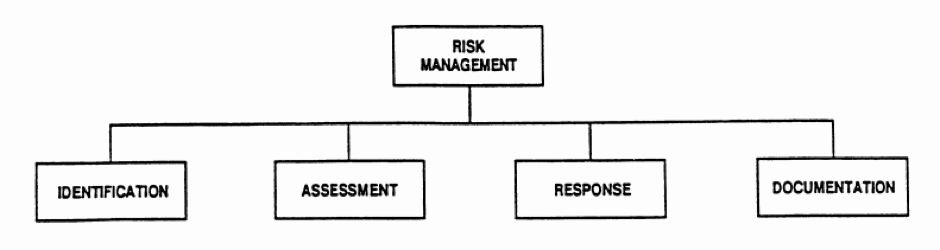
\includegraphics[scale=0.80]{EAP_Gerenciamento_de_Riscos.png}
		\caption{Etapas do plano de gerenciamento de riscos segundo Max \cite{wideman1992project}}
		\label{img:eap_gerenciamento_de_risco}
		\end{figure}
	
	\begin{itemize}
	 \item \textbf{Identificação}: Esta fase consiste em identificar todos os possíveis riscos que podem impactar de forma severa o sucesso do projeto. Os tipos de impacto podem variar dependendo de onde ele afeta no projeto e quais as probabilidades deles acontecerem. Combinações de riscos que juntos podem representar uma ameaça mais do que individualmente não podem ser ignorados.
	 \item \textbf{Avaliação}: Tendo identificado todo o alcance de riscos possíveis o próximo passo é os avaliar. O propósito é determinar os atributos do erro como o impacto, probabilidade e tipo de erro.
	\item \textbf{Resposta}: A parte de mitigação de riscos no projeto consiste em estabelecer uma estratégia de sistema apropriada, assim garantindo uma abordagem apropriada aos riscos caso eles venham a acontecer. Nesta etapa é descrito qual será a reação da equipe para tratar algum tipo de risco caso ele venha a acontecer.
	\item \textbf{Documentação}: Documento final e vital para o projeto que detalha todos os riscos, com suas características e quais serão as ações tomadas pela equipe de forma detalhada,caso cada risco apontado chegue a acontecer.
	\end{itemize}

	\subsection{EAR - Estrutura Analítica de Riscos para identificação dos riscos}
	O Project Management Institute (PMI), instituto que elaborou o Project Management Book of Knowledge (PMBoK) \cite{pmbok2012}, possui um template de estrutura analitica de riscos que possui as seguintes categorias e sub-divisões: 
	
	\graphicspath{{figuras/}}
	\begin{figure}[h!]
	\centering
	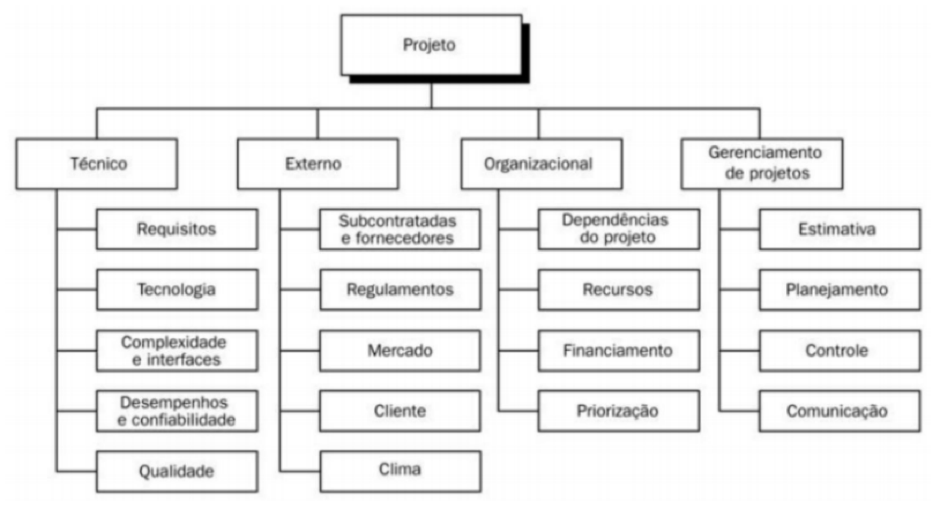
\includegraphics[scale=0.80]{classificacao_de_riscos.png}
	\caption{Classificação dos riscos na EAR segundo o PMI}
	\label{img:classificacao_de_riscos}
	\end{figure}
	
	\graphicspath{{figuras/}}
	\begin{figure}[h!]
	\centering
	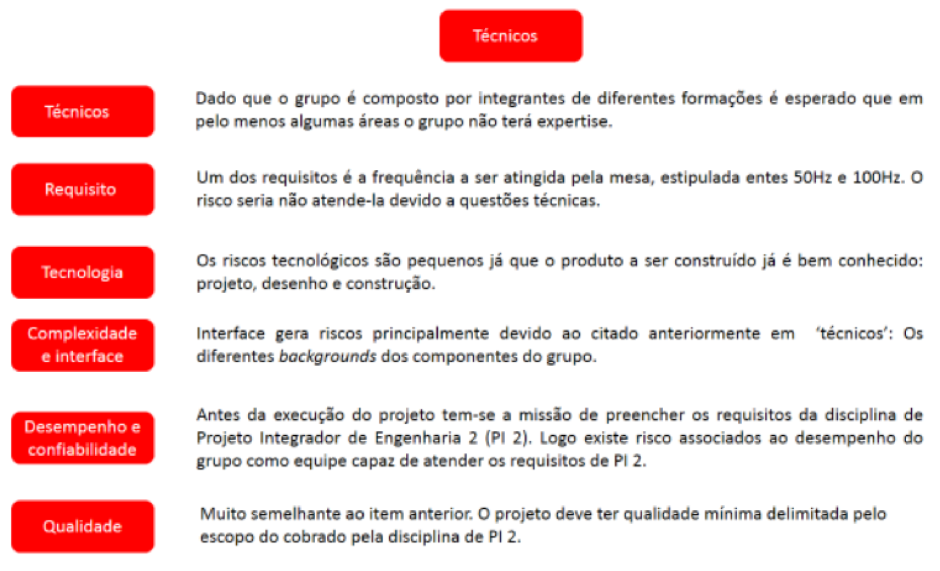
\includegraphics[scale=0.80]{analise_riscos_tecnicos.png}
	\caption{Análise em relação aos riscos técnicos}
	\label{img:analise_riscos_tecnicos}
	\end{figure}
	
	\graphicspath{{figuras/}}
	\begin{figure}[h!]
	\centering
	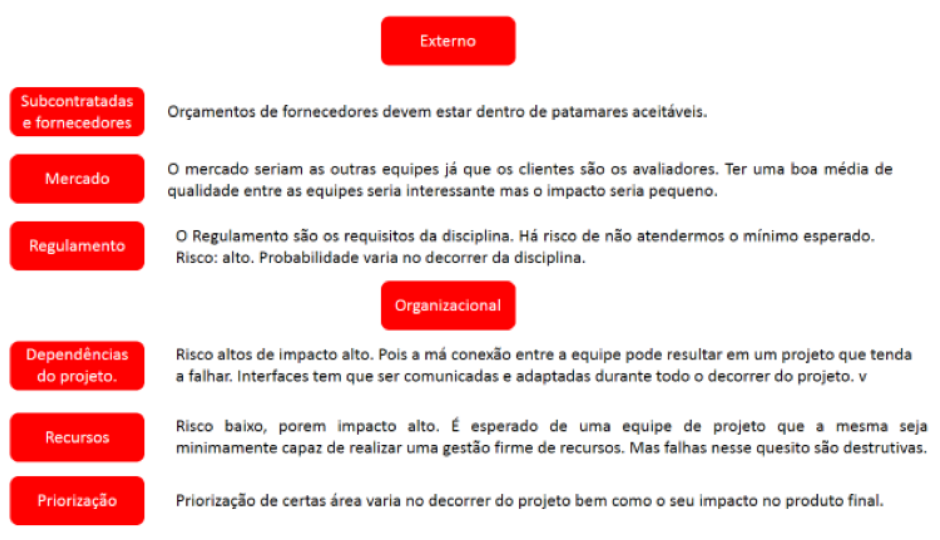
\includegraphics[scale=0.80]{analise_riscos_externos.png}
	\caption{Análise em relação aos riscos externos e organizacionais}
	\label{img:analise_riscos_externos}
	\end{figure}	
	
	\subsection{Qualificação dos Riscos}
	Os riscos identificados pelo grupo foram qualificados de acordo com sua probabilidade de ocorrência e o impacto resultante no projeto. O sistema de probabilidade e impactos foram classificados de acordo com a tabela padronizada do Gantter (ferramenta de gerenciamento de riscos adotada pela equipe).
	
	\begin{table}[h!]
\centering
\caption{Probabilidade dos Riscos}
\label{tabela_probabilidade_riscos}
\begin{tabular}{|ll|}
\hline
\multicolumn{1}{|l|}{\textbf{Nível}} & \textbf{Probabilidade} \\ \hline
Improvável                           & 0\% $\sim$ 20\%        \\
Remoto                               & 21\% $\sim$ 40\%       \\
Ocasional                            & 41\% $\sim$ 60\%       \\
Provável                             & 61\% $\sim$ 80\%       \\
Frequente                            & 81\% $\sim$ 100\%      \\ \hline
\end{tabular}
\end{table}	

\begin{table}[h!]
\centering
\caption{Severidade dos Riscos}
\label{tabela_severidade_de_riscos}
\begin{tabular}{|ll|}
\hline
\multicolumn{1}{|l|}{\textbf{Nível}} & \textbf{Descrição}                                                                                                                                                             \\ \hline
Negligível                           & Risco que não afeta a integridade do projeto de forma a comprometer o mesmo.                                                                                                   \\ \hline
Baixo                                & Possui pouco prejuízo ao desenvolvimento do projeto.                                                                                                                           \\ \hline
Moderado                             & \begin{tabular}[c]{@{}l@{}}Prejudica o desenvolvimento do projeto. Pode ser resolvido\\ em um curto período de tempo.\end{tabular}                                             \\ \hline
Significante                         & \begin{tabular}[c]{@{}l@{}}Prejudica o desenvolvimento do projeto. Gasta-se um tempo significativo\\ (semanas) para conseguir restituir a integridade do projeto.\end{tabular} \\ \hline
Catastrófico                         & Erro que previne o projeto de ser concluído.                                                                                                                                   \\ \hline
\end{tabular}
\end{table}
	
	\subsection{Prioridade dos Riscos}
	A prioridade dos riscos também foi feita de acordo com as opções já padronizadas da ferramenta “Gantter”, sendo elas:
	
	\begin{table}[h!]
\centering
\caption{Prioridade dos Riscos}
\label{tabela_prioridade_dos_riscos}
\begin{tabular}{|ll|}
\hline
\multicolumn{1}{|l|}{\textbf{Nível}} & \textbf{Descrição}                                                                                                                                                                                                                  \\ \hline
Sem Ação                             & O risco é tão pequeno ou irrelevante que nenhuma ação será tomada.                                                                                                                                                                  \\ \hline
Monitorar                            & \begin{tabular}[c]{@{}l@{}}O risco possui um certo grau de causar problemas, sendo \\ monitorado constantemente.\end{tabular}                                                                                                       \\ \hline
Tomar Ação                           & \begin{tabular}[c]{@{}l@{}}O risco possui uma boa probabilidade de causar problemas no projeto \\ e devem ser tomadas medidas de mitigação para que o mesmo não \\ aconteça ou reduza seu impacto.\end{tabular}                     \\ \hline
Ação Urgente                         & \begin{tabular}[c]{@{}l@{}}O risco possui uma boa probabilidade de causar muitos problemas no \\ projeto e devem ser tomadas medidas prioritárias de mitigação para que\\  o mesmo não aconteça ou reduza seu impacto.\end{tabular} \\ \hline
Interromper Projeto                  & \begin{tabular}[c]{@{}l@{}}O risco é tão significante que se interrompe o projeto até que seja \\ encontrada uma forma de contornar tal erro.\end{tabular}                                                                          \\ \hline
\end{tabular}
\end{table}	
	
	\subsection{Riscos Identificados}
	Os riscos identificados para o projeto estão listados na Tabela \ref{riscos_identificados}

\begin{table}[h!]
\centering
\caption{Riscos Identificados}
\label{riscos_identificados}
\begin{tabular}{|llll|}
\hline
\multicolumn{1}{|l|}{\textbf{Risco}}       & \multicolumn{1}{l|}{\textbf{Probabilidade}} & \multicolumn{1}{l|}{\textbf{Severidade}} & \textbf{Prioridade} \\ \hline
Trancamento de um integrante do grupo      & Remoto                                      & Moderada                                 & Monitorar           \\ \hline
Atraso nas entregas das atividades         & Provável                                    & Significante                             & Ação Urgente        \\ \hline
Desentendimento entre os membros da equipe & Ocasional                                   & Baixa                                    & Monitorar           \\ \hline
Atraso na entrega de um produto/serviço    & Ocasional                                   & Significante                             & Ação Urgente        \\ \hline
Problemas com a API                        & Remoto                                      & Catastrófica                             & Ação Urgente        \\ \hline
Vibração do motor                          & Remoto                                      & Baixa                                    & Monitorar           \\ \hline
Aquecimento dos componentes                & Remoto                                      & Moderada                                 & Monitorar           \\ \hline
Ergonomia do produto                       & Remoto                                      & Baixa                                    & Monitorar           \\ \hline
Custo inviável                             & Remoto                                      & Significante                             & Monitorar           \\ \hline
Atraso/falta dos integrantes nas reuniões  & Remoto                                      & Moderada                                 & Tomar Ação          \\ \hline
\end{tabular}
\end{table}

	\subsection{Ação de Resposta aos Riscos}
	As ações que foram definidas pelo time à serem tomadas para cada risco identificado se encontram na Tabela \ref{acoes_de_resposta}.

\begin{table}[!h]
\centering
\caption{Ações de Respostas aos Riscos}
\label{acoes_de_resposta}
\begin{tabular}{|ll|}
\hline
\multicolumn{1}{|l|}{\textbf{Risco}}       & \textbf{Resposta}                                                                                        \\ \hline
Trancamento de um integrante do grupo      & \begin{tabular}[c]{@{}l@{}}Redistribuir as atividades entre os \\ membros da mesma equipe\end{tabular}   \\ \hline
Atraso nas entregas das atividades         & \begin{tabular}[c]{@{}l@{}}Realinhar o cronograma e atuação do \\ responsável por tal grupo\end{tabular} \\ \hline
Desentendimento entre os membros da equipe & Alinhamento de idéias através dos líderes                                                                \\ \hline
Atraso na entrega de um produto/serviço    & \begin{tabular}[c]{@{}l@{}}Reunião dos líderes e tomada de ação no \\ setor com problemas\end{tabular}   \\ \hline
Problemas com a API                        & Procurar uma nova API                                                                                    \\ \hline
Vibração do motor                          & Procurar uma solução melhor                                                                              \\ \hline
Aquecimento dos componentes                & Replanejamento da estrutura                                                                              \\ \hline
Ergonomia do produto                       & Replanejamento da estrutura                                                                              \\ \hline
Custo inviável                             & Replanejamento dos componentes                                                                           \\ \hline
Atraso/falta dos integrantes nas reuniões  & \begin{tabular}[c]{@{}l@{}}Comunicação entre os representantes do \\ grupo com o indivíduo\end{tabular}  \\ \hline
\end{tabular}
\end{table}
	
	\subsection{Sistema de Controle de Mudanças de Riscos}
	O sistema serve justamente para alinhar a equipe sobre os riscos que o projeto pode vir a ter em seu decorrer e quais serão as ações que devem ser tomadas para cada tipo. A equipe deve estar consciente da probabilidade de cada risco encontrado a fim de controlar e manter o progresso do projeto em um meio que o risco possa sempre ser evitado.

	Cada risco não encontrado pelo grupo na fase de elaboração do projeto deverá ser documentado neste documento no futuro segundo os padrões adotados pela equipe e da ferramenta usada por ela para gerenciamento de riscos.

	
	\chapter{Plano de Custos}

	
	\chapter{Cronograma Detalhado}
		\subsection{Ponto de Controle 1}
		As atividades do Ponto de Controle 1 estão representadas na figura \ref{img:PC1}. As atividades foram divididas em cinco subgrupos que são:

		\begin{itemize}
			\item Gerência;
			\item Software;
			\item Alimentação;
			\item Eletroeletrônica;
			\item Estrutura;
		\end{itemize}	
		
		\graphicspath{{figuras/}}
			\begin{figure}[h!]
			\centering
			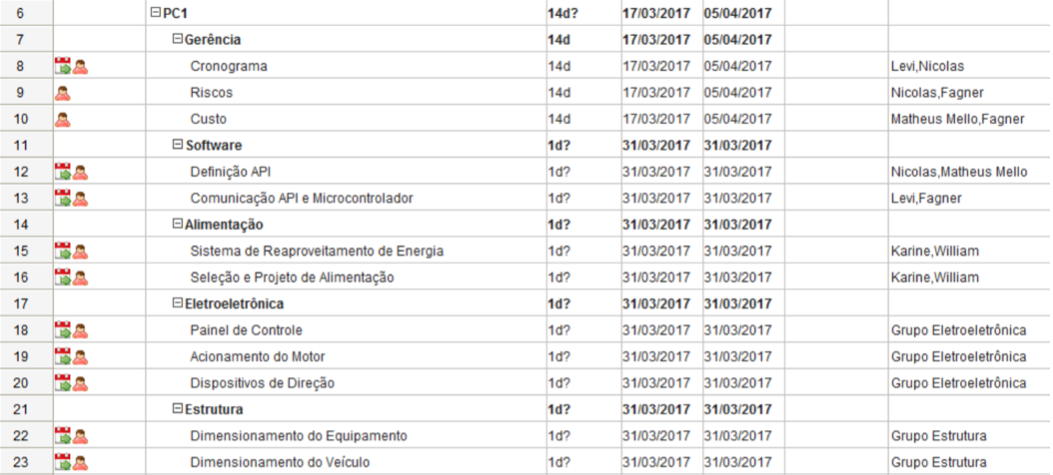
\includegraphics[scale=0.60]{PC1}
			\caption{Atividades do Ponto de Controle 1}
			\label{img:PC1}
			\end{figure}	
		
		As atividades do subgrupo de Gerência são:
		
		\begin{itemize}
			\item \textbf{Cronograma}: criação de um cronograma, contendo as datas de início e fim das atividades e os seus respectivos responsáveis.
			\item \textbf{Riscos}: definição dos riscos do projeto.
			\item \textbf{Custo}: levantamento dos custo do projeto, definindo a prioridade de aquisição.
		\end{itemize}	
		
		As atividades do subgrupo de Software são:
		
		\begin{itemize}
			\item \textbf{Definição API}: definir qual API será utilizada para implementação da solução de software.
			\item \textbf{Comunicação API e Microcontrolador}: definir a forma mais viável de transferir as informações coletadas pela API para o microcontrolador.
		\end{itemize}				

	As atividades do subgrupo de Alimentação são:
	
	\begin{itemize}
		\item \textbf{Sistema de Reaproveitamento de Energia}: definir um mecanismo que possa ser reaproveitar a energia e utiliza-lá para alimentação dos componentes eletrônicos.
		\item \textbf{Seleção e Projeto de Alimentação}: definir a melhor solução para alimentar o sistema. 
	\end{itemize}		
	
	As atividades do subgrupo de Eletroeletrônica são:
	\begin{itemize}
		\item \textbf{Painel de Controle}: definir o funcionamento do painél de controle acoplado à bicicleta para que se tenha informações do sistema.
		\item \textbf{Acionamento do Motor}: definir como será feito o acionamento do motor utilizando componentes eletrônicos.
		\item \textbf{Dispositivos de Direção}: definir os dispositivos de navegação que serão utilizados juntamente com a API de direção.
	\end{itemize}

	As atividades do subgrupo de Estrutura são:
	\begin{itemize}
		\item \textbf{Dimensionamento do Equipamento}: definir como serão acoplados os componentes eletrônicos ao sistema.
		\item \textbf{Dimensionamento do Veículo}: definir o desenho do veículo.
	\end{itemize}

	\subsection{Ponto de Controle 2}
		As atividades do Ponto de Controle 2 estão representadas na figura \ref{img:PC2}. As atividades foram divididas em quatro subgrupos que são:

		\begin{itemize}
			\item Software;
			\item Alimentação;
			\item Eletroeletrônica;
			\item Estrutura;
		\end{itemize}	
		
		\graphicspath{{figuras/}}
			\begin{figure}[h!]
			\centering
			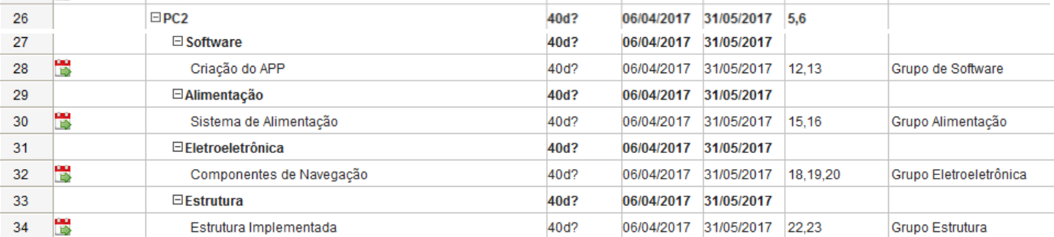
\includegraphics[scale=0.60]{PC2}
			\caption{Atividades do Ponto de Controle 2}
			\label{img:PC2}
			\end{figure}	
			
			As atividades do subgrupo de Software são:
			
			\begin{itemize}
				\item \textbf{Criação do APP}: implementar o app que fará a comunicação com o microcontrolador
			\end{itemize}
			
			As atividades do subgrupo de Alimentação são:
			\begin{itemize}
				\item \textbf{Sistema de Alimentação}: implementar o sistema que alimentará o veículo.
			\end{itemize}
			
			As atividades do subgrupo de Eletroeletrônica são:
			\begin{itemize}
				\item \textbf{Componentes de Navegação}: implementar o sistema de navegação que será acoplado ao veículo
			\end{itemize}
			
			As atividades do subgrupo de Estrutura são:
			\begin{itemize}
				\item \textbf{Estrutura Implementada}: implementar a estrutura do veículo.
			\end{itemize}
			
			\subsection{Ponto de Controle 3}
			As atividades do Ponto de Controle 2 estão representadas na figura \ref{img:PC3}.
		
		\graphicspath{{figuras/}}
			\begin{figure}[h!]
			\centering
			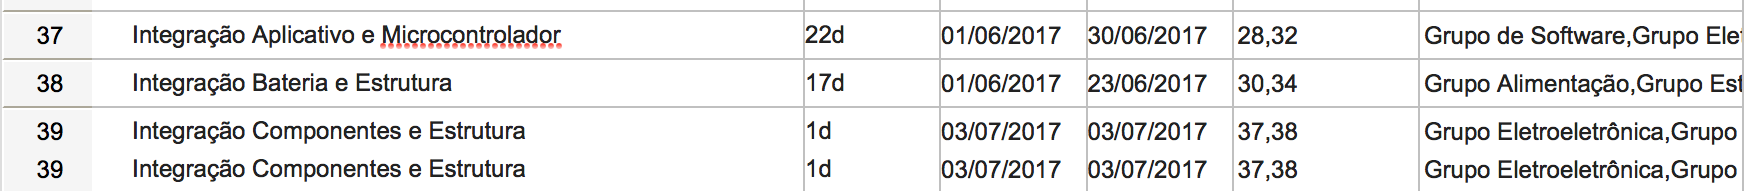
\includegraphics[scale=0.60]{PC3}
			\caption{Atividades do Ponto de Controle 3}
			\label{img:PC3}
			\end{figure}
			
			As atividades são:
			
			\begin{itemize}
				\item \textbf{Integração Aplicativo e Microcontrolador}: fazer a integração das duas interfaces e garantir o funcionamento do sistema.
				\item \textbf{Integração Bateria e Estrutura}: fazer o acoplamento da bateria à estrutura e garantir o funcionamento do sistema.
				\item \textbf{Integração Componentes e Estrutura}: fazer o acoplamento final entre os componentes e a estrutura (que já se encontra com a bateria), e garantir o funcionamento do sistema.
				\item \textbf{Teste de Integração}: teste que é feito ao fim de cada integração para garantir o funcionamento do sistema.
				\item \textbf{Teste Final}: teste feito ao fim de todas as integrações, onde o produto já foi finalizado. 
			\end{itemize}
			
			
			
			
%\end{comment}

\chapter{Estrutura}
\label{estrutura}
	\section{Desenho técnico do gabarito da adaptação}
	\label{gabarito}
		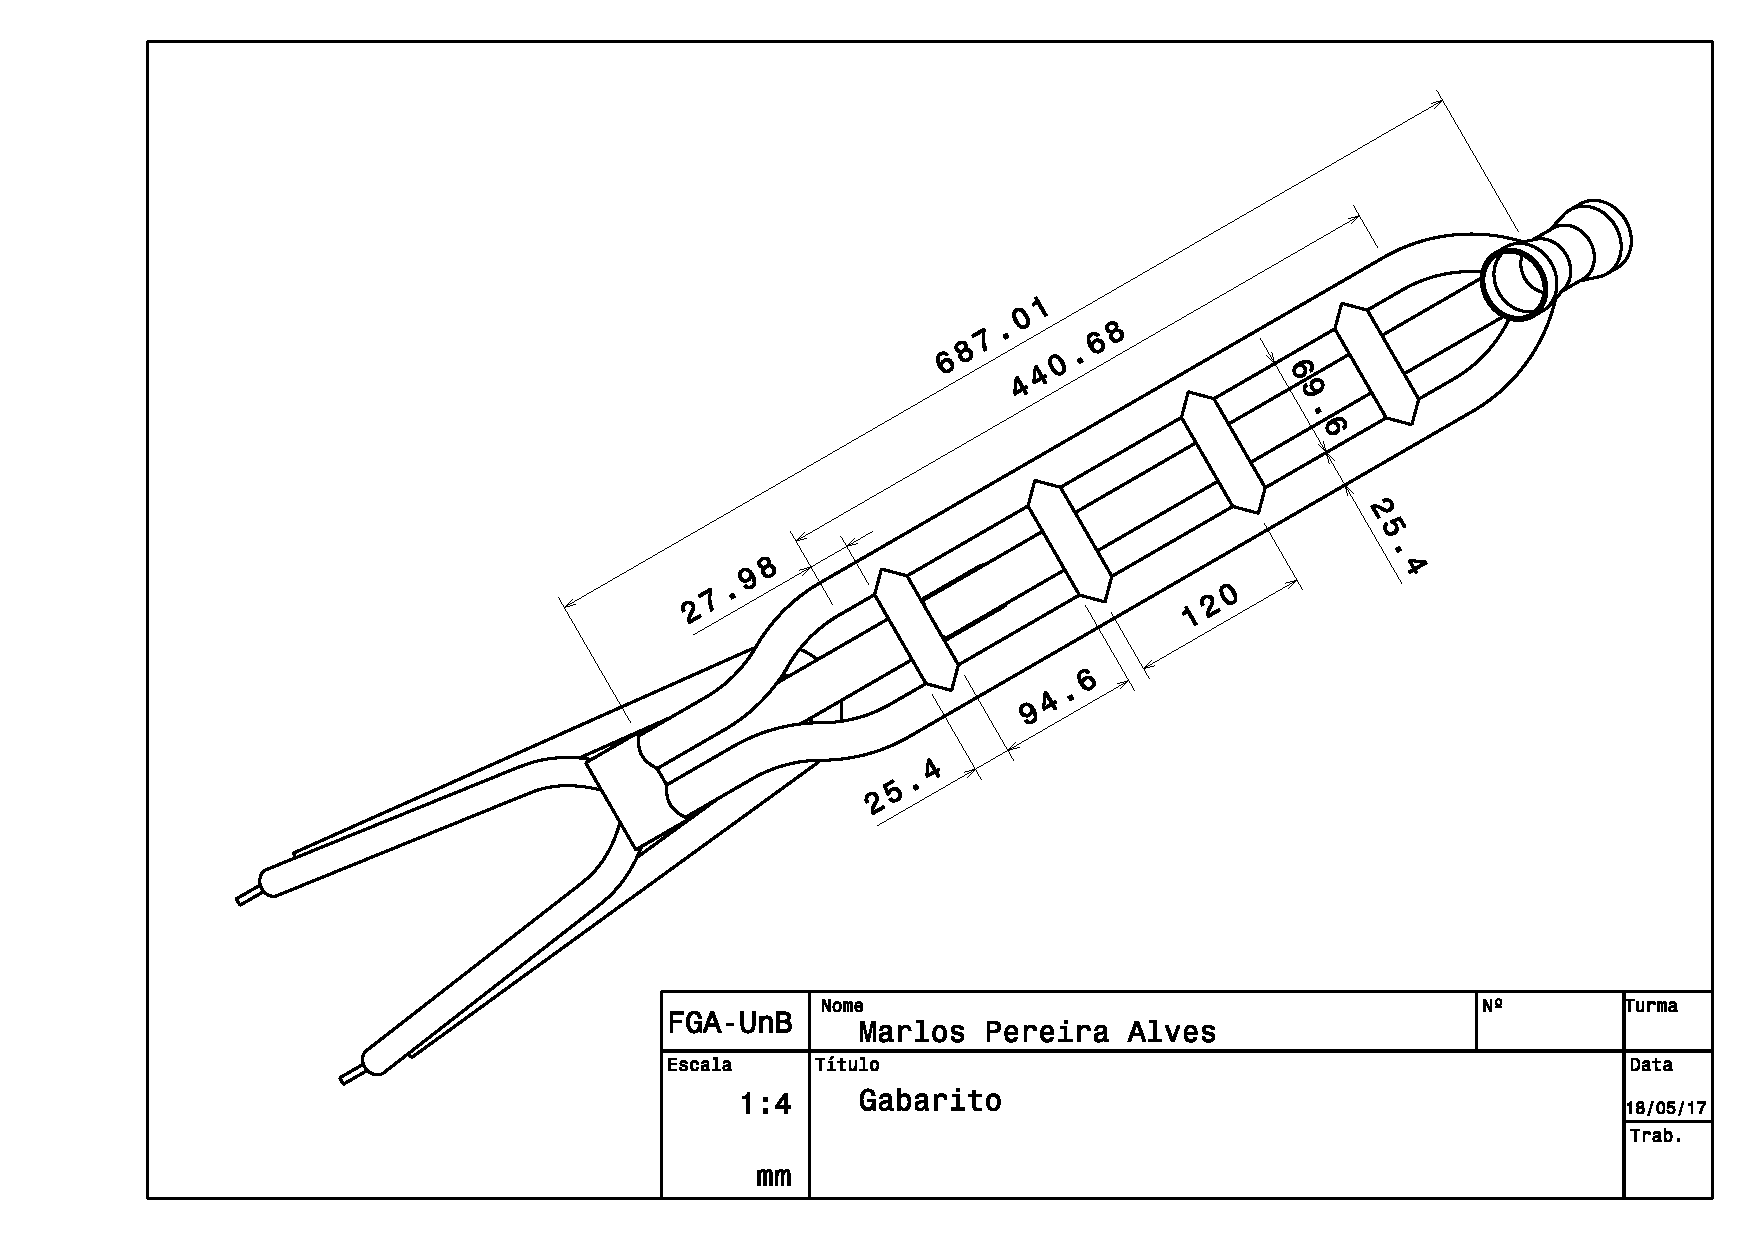
\includepdf[landscape]{Bike_v4.pdf}

\chapter{Relatórios Individuais}
	\label{relatorios}
	\begin{itemize}
		\item \textbf{Matheus Mello Nascimento - 11/0017692} - Atuei desde  a definição do processo estabelecido para o desenvolvimento da aplicação de software, até o desenvolvimento em si, trabalhei na parte da aplicação WEB e no aplicativo, na comunicação com a API de geolocalização do Google Maps e com a integração Bluetooth utilizando o módulo HC-06 em conjunto com o arduíno.
		
		\item \textbf{Paulo Henrique Bernardo Melo - 09/0011996} - Dentro das tarefas da engenharia eletrônica trabalhei na escolha e implantação dos circuitos e sensores responsáveis por medir o nível da bateria e a velocidade desenvolvida pela bicicleta, bem como no código em arduíno que filtra o sinal e os envia aos displays o-leds. Auxiliei na construção do sistema de visualização de rota pelo usuário por meio dos displays o-led com o interfaceamento com o microcontrolador, criando um protocolo, e juntando as informações provenientes do módulo bluetooth vindos da aplicação WEB através de um código desenvolvido no arduíno. Ademais, ajudei na escrita do trabalho, na integração das partes, e na compra dos componentes.
		
		\item \textbf{Bruno Fernandes Fares - 09/0003993} - O grupo de Engenharia Eletrônica foi dividido em duas frentes, onde fiquei responsável pela parte de Sistema de Controle e integração com o grupo de Software. Implementei os códigos e bibliotecas em arduino responsáveis pela coleta dos dados do bluetooth e do sensor de velocidade, além do processamento das imagens a serem geradas no par de displays O’led. Além disso, junto ao pessoal de software, auxiliei na parte do aplicativo responsável por se comunicar com o módulo bluetooth e entreguei a eles o protocolo completo de comunicação. Por fim, como parte da integração com estrutura, atuei na confecção das placas e concepção da caixa acopladora.
		
		\item \textbf{Lúcio César Pimenta Luiz- 11/0035216 }- Envolvi-me na criteriosa seleção do modelo e estilo da bicicleta, além de seus materiais e componentes. Também fui responsável pela análise estática e de estabilidade da Unbike, feita de forma ergonômica.
		Por fim, participei de todo o processo de construção da caixa do produto.
		
		\item \textbf{Marlos Pereira Alves - 11/0064143} - Na fase de pré-projeto, contribui na escolha do modelo base  adotado na adaptação, modelei em ambiente CAD a adaptação do quadro, realizei as análises estáticas em MEF em plataforma CAE do software Ansys, ajudei na escolha do material e espessura dos tubos, levantei orçamentos de materiais e de profissionais capazes de realizar solda em alumínio, e fui responsável pela compra dos tubos de alumínio. Na fase de construção, participei da confecção da adaptação, do compartimento principal, da caixa de baterias e da fixação no quadro adaptado.No que tange o relatório final, ajudei na sua confecção e cooperei na edição e organização do trabalho em LaTeX/GitHub.
		
		\item\textbf{ Matheus Kiyoshi Silva Alimura - 12/0129841}- Participei de todo o processo de seleção do tipo de bicicleta que seria implementado, das características necessárias, pesquisa de mercado até a seleção da bicicleta e sua compra. Ajudei na fabricação da peça que foi modificada no quadro da bicicleta. Modelei em CAD o compartimento das baterias e o compartimento principal, e participei da compra dos materiais, da construção e fixação dos dois compartimentos, e pintei o compartimento principal. Na parte do relatório, contribui para a sua produção no que diz respeito a frente de estrutura.
		
		\item \textbf{Ricardo de Castro Paranhos – 12/0021552} – Minha contribuição para o projeto foi dimensionar o banco de baterias para alimentar todo o sistema. Auxiliei a frente de eletrônica na parte de acionamento do motor, uma vez que a mesma placa de acionamento e controle do motor é utilizada para a regeneração de energia. Comprei todos os materiais necessários para a confecção do carregador das baterias e o fiz: estrutura de madeira, transformador abaixador com ponte retificadora, circuito abaixador de tensão, pintura da caixa. Realizei teste para a regeneração de energia e auxiliei na integração. 
		
		\item \textbf{William de Oliveira Medeiros - 11/0021738} - Dentro da minha área de Alimentação, participei do processo de dimensionamento e compra das baterias para alimentação do sistema. Além disso, com a posterior necessidade de se regenerar energia através do motor, atuei auxiliando o subgrupo de Eletrônica responsável pela placa de acionamento/regeneração, ajudando que ela ficasse adequada a nova necessidade. Por fim, fiz a simulação do circuito de carregamento das baterias, verificando e dimensionando os componentes diversos para as necessidades exigidas, além de participar da confecção do circuito em si e da caixa de madeira que o comporta. Externamente a meu subgrupo, participei da confecção do suporte de madeira das baterias junto ao subgrupo de Estrutura. 
		
		\item \textbf{Fagner Rodrigues - 09/0112750} - Atuei no projeto inicialmente como na base da engenharia de software, realizando o levantamento e definição dos requisitos de software, definição da arquitetura do sistema, realizei o desenvolvimento da aplicação de software tais como cadastro e acesso de usuário, visualização de perfil de usuário, e na integração Bluetooth em conjunto com o arduíno para o envio dos dados relacionados às rotas, parte desenvolvida juntamente com o integrante Matheus Mello. Além do desenvolvimento da parte de software em si, realizei contribuições com ajuda para a implementação circuito de acionamento e controle de aceleração do motor e construção da caixa de suporte de baterias e circuitos.
		
		\item \textbf{Levi Moraes - 11/0015339} - Inicialmente estava ajudando nas definições de algumas decisões referentes ao software que seria utilizado no app.Trabalhei também na melhoria do processo de desenvolvimento do software. Após o segundo ponto de controle, pelo fato de a maior parte do software já ter sido desenvolvida, ajudei em algumas questões de integração do módulo bluetooth com o app, porém passei mais tempo ajudando as outras frentes.
		
		\item \textbf{Nicolas Boarin - 11/0064879}  - Participei desde a criação da ideia e decisão dos integrantes dos grupos inicialmente. Fazendo parte do grupo de software e idealizador da ideia, ajudei nas definições e na tomada de decisões de que rumo o software deveria tomar chegando no produto final. Junto com o Levi formamos a frente da melhoria de processo de desenvolvimento de software. Também fiquei encarregado do levantamento e distribuição de recursos para manter o projeto como tesoureiro. Com o software pronto já para integração meus trabalhos continuaram como tesoureiro e ajudando outras frentes com trabalhos manuais de suporte.
	\end{itemize}
\end{apendicesenv}
